%protocol.tex

\subsection{Overview}
%
%% This section describes the Synapse protocol.
We now present our generic \emph{meta}-protocol for information
distribution and retrieval over an interconnection of heterogeneous
overlay networks. Information is a set of basic {\tt (key, value)}
pairs, as commonly encountered in protocols for information retrieval.

The protocol specifies how to insert information ({\tt PUT}), how to
retrieve it through a key ({\tt GET}), how to invite nodes in a given
overlay ({\tt INVITE}), and how to join a given overlay ({\tt JOIN})
over a heterogeneous collection of overlay networks linked by
co-located nodes. These co-located nodes
%% are the possibility of bridges between the overlays, and
represent a simple way to aggregate the resources of distinct
overlays. We assume each overlay to have its own inner routing
algorithm, called by the Synapse protocol to route requests inside
each overlay. We assume no knowledge about the logical topology of all
the involved overlay networks connected by Synapse. To ensure the
usual properties of the underlying network, we assume that
communication is both symmetric and transitive. Synapse simply ignores
about how routing takes place inside the overlays, Synapse only offers
a mechanism to route from one overlay to another in a simple, scalable
and efficient way.

One important requirement of the Synapse protocol with respect to
others protocols using hash functions, is that keys and nodes'
addresses circulate \emph{unhashed} from hop to hop. Recall that hash
function have no inverse: once a sought key is hashed, it is
impossible its initial value and this impossible to forward to another
overlay having a different hash function, since hash functions can be
different (in implementations and keysize) from overlay to overlay.

Obviously, both the hashed and the \emph{clear} key data can be
carried in the message or a fast hash computation can be performed at
each step. Standard cryptographic protocols can be used in case of
strong confidentiality requirements without affecting the scalability
of the Synapse protocol itself.

%%% �a c pas de l'overview, c super pr�cis !!
More precisely, the initialization of a search query is done via the
following steps: The initiator $(i)$ logs the message in the node,
$(ii)$ sets a TTL and $(iii)$ launches a {\tt FIND} message in a first
overlay. Upon receipt of a {\tt FIND} message, a node checks first if
the TTL is valid and second if this query was already processed on the
node: in both cases, the routing aborts, in order to avoid useless
message overhead.

\begin{figure*}[!t]
{\scriptsize
\begin{alltt}
\AL \textbf{on receipt of} OPE(code,key,value) \textbf{from} ipsend \textbf{do}\alglabel{alg:ope}\hfill{\rm receive an operation code a key and a value from ipsend}
\AL  tag = this.new_tag(ipsend);\hfill{\rm create a new unique tag for this lookup}
\AL  \textbf{send} FIND(code,ttl,mrr,tag,key,value,ipsend) \textbf{to} this.myip;\alglabel{alg:ope_end}\hfill{\rm send a FIND message with code, ttl, mrr, tag, key, value and ipsend to itself}
\NA
\AL \textbf{on receipt of} FIND(code,ttl,mrr,tag,key,value,ipdest)\textbf{from} ipsend \textbf{do}\alglabel{alg:find}\hfill{\rm receive a FIND message with code, ttl, mrr ... ipdest from ipsend}
\AL   \textbf{if} ttl = 0 or this.game_over?(tag)\hfill{\rm the lookup is aborted because of zero ttl or because of the game over strategy}
\AL   \textbf{else} this.push_tag(tag); \hfill{\rm push the tag of the query as ``already processed''}
\AL     next_mrrs = distrib_mrr(mrr,this.net_list); \alglabel{alg:mrr}\hfill{\rm fix the associative list splitting all the mrr between all net the synapse belongs to}
\AL     \textbf{for all} net\( \in \)this.net_list \textbf{do}\hfill{\rm for all net the synapse belongs do}
\AL       \textbf{if} this.isresponsible?(net,key) \alglabel{alg:test}\hfill{\rm the current synapse is responsible for the key in the net}
\AL         \textbf{send} FOUND(code,net,mrr,key,value) \textbf{to} ipdest; \alglabel{alg:send_found}\hfill{\rm send a FOUND message with code, net, mrr, key and value to ipdest}
\AL       \textbf{else if} this.good_deal?(net,ipsend)\hfill{\rm the net/ipsend is a  ``good'' net/synapse  (left to synapse's strategy)}
\AL              \textbf{send} FIND(code,ttl-1,next_mrr.get(net),tag,key,value,ipdest) \textbf{to} this.next_hop(key);\alglabel{alg:find_end}\hfill{\rm send a FIND msg with ... to ...}
\NA
\AL \textbf{on receipt of} FOUND(code,net,mrr,key,value) \textbf{from} ipsend\alglabel{alg:found}\textbf{do}\hfill{\rm receive a FOUND message with code, net, key and value from ipsend}
\AL   this.good_deal_update(net,ipsend);\hfill{\rm update my good deal tables with net and ipsend}
\AL   \textbf{match} code
\AL    code=GET  \alglabel{alg:get_code}\hfill{\rm GET code}
\AL     \textbf{send} READ_TABLE(net,key) \textbf{to} ipsend \alglabel{alg:get_code_end}\hfill{\rm send a READ\_TABLE message (omitted) through the net with key to ipsend}
\AL    code=PUT \alglabel{alg:put_code}\hfill{\rm PUT code}
\AL     \textbf{if} mrr < 0 \hfill{\rm stop replication since no inter PUT is allowed}
\AL     \textbf{else} \textbf{send} WRITE_TABLE(net,key,value) \textbf{to} ipsend \alglabel{alg:put_code_end}\hfill{\rm send a WRITE\_TABLE message (omitted) through the net with key and value to ipsend}
\NA
\AL \textbf{on receipt of} INVITE(net) \textbf{from} ipsend \textbf{do} \alglabel{alg:join_req}\hfill{\rm receive an invitation to join the net from ipsend}
\AL   \textbf{if} this.good_deal?(net,ipsend)\hfill{\rm the net/ipsend is a  ``good'' net/synapse (left to peer's strategy)}
\AL     \textbf{send} JOIN(net) \textbf{to} ipsend; \alglabel{alg:join_req_end} \hfill {\rm send a JOIN message to reach the net to ipsend}
\NA
\AL \textbf{on receipt of} JOIN(net) \textbf{from} ipsend\alglabel{alg:join_req_ok}\textbf{do}\hfill{\rm receive a JOIN message to reach the net from ipsend}
\AL   \textbf{if} this.good_deal?(net,ipsend)\hfill{\rm  the net/ipsend is a  ``good'' net/synapse (left to synapse's strategy)}
\AL     this.insert_net(net,ipsend);\alglabel{alg:join_req_ok_end}\hfill{\rm the current synapse insert ipsend in the net}
\end{alltt}}
\caption{The Synapse protocol \label{fig:lookup}}
\end{figure*}


% \AL    code=LEAVE\hfill{\rm LEAVE code}
% \AL    this.references.delete(f,ipsender);\hfill{\rm delete references with ipsender at floor f}
% \AL    \textbf{send} LEFT!(f) \textbf{to} ipsender;\hfill {\rm  the peer ipsender has left f}
% \AL    code=INVITE  \alglabel{alg:discover_code}\hfill{\rm INVITE code}
% \AL    \textbf{if} this.good_deal?(net,ipsend)\hfill{\rm the peer ipsend and the network net are ``good'' (peer's strategy)}
% \AL    \textbf{send} JOIN(net) \textbf{to} ipsend;\alglabel{alg:discover_code_end}\alglabel{alg:found_end}\hfill {\rm the peer ipsend want to join the network net}



\subsection{Architecture and Assumptions}
%
The inter-overlay network, induced by the Synapse protocol, can be
considered as an aggregation of heterogeneous sub-overlay natworks
(referred to as \emph{intra}-overlay networks henceforth).  Each
intra-overlay consists of one instance of, \eg, Chord or any structured,
unstructured or hybrid overlay. We recall that an overlay network for
information retrieval consists of a set of nodes on which the
information on some resources (collection of ({\tt key,value}) pairs)
is distributed. Each intra-overlay has its own key/value distribution
and retrieval policy, logical topology, search complexity, routing and
fault-tolerance mechanisms , so on and so forth. The Synapse protocol
can be summarized by the following points:
%
\begin{maliste}

\item {\em Synapses:} the interconnection of intra-overlay networks is
  achieved by co-located nodes taking part in several of these
  intra-overlays, called synapses. Each peer will act according to the policy
  of each of its intra-overlays, but will have the extra-role of
  forwarding the requests to some intra-overlay it belongs to.

\item {\em Peer's name:} every peer comes with a proper logical name
  in each intra-overlay; in particular, synapses have as many
  logical names as the number of networks they belongs to.

\item {\em Keys mapping in peers:} each peer is responsible for a set
  of resources ({\tt key,value}) it hosts. Since every
  intra-overlay have different policies for keys distribution, we
  could say that also the inter-overlay induced by Synapse inherits an
  homogeneous distribution among the intra- and inter-networks. As for
  peers, every key comes with a proper logical name peculiar to each
  intra-overlay.

\item {\em Set of resources assigned to set of nodes:} all overlays
 protocol for information retrieval share the invariant of having a set of peers
 responsables of a specific set of resources. This invariant allows
 to route under structured, unstructured and hybrid networks: the
 rationale is simple: by construction, ever intra-routing is
 responsible for its correctness, since Synapse just care about
 overlay's inter-connection.

\item {\em Network independency and message translation:}
 intra-network protocols are different by construction: as such, when
 a message leaves a particular network and enters another network, the
 first network looses the control on the route taken inside the second one.

\item {\em Topology, exhaustiveness, complexity and scalability:} by
 construction, the inter-overlay network induced by the Synapse
 protocol belongs to the category of unstructured overlay networks,
 with a routing that is not exhaustive, even if Synapse can connect
 only overlays that guarantee exhaustivity. The same goes for the
 routing complexity that can be upper-bounded only in presence of
 precise and strong hypotheses about the type of intra-overlay
 networks. The same for scalability: a Synapse inter-network is
 scalable if all the intra-networks are scalable.


  % FRANCESCO : SI TU VEUX LE CASER QUELQUE PART... => non
  % As example, if we consider only Chord
  % overlay networks, it is worth to observe that while the search within
  % a single Chord ring is \emph{exhaustive} and \emph{logarithmic} in
  % the number of peers, the whole lookup in Synapse \emph{can be non
  %   exhaustive} with a routing complexity that can vary according to
  % the \emph{number of Chord networks} (inter-net routing) \emph{times
  %   a logarithmic factor} (intra-net routing).

  % FRANCESCO : SI TU VEUX LE CASER QUELQUE PART... => et non , on se r�p�te
  % A nice property of
  % Synapse's routing mechanisms is that with a fairly low amount of
  % synapses, we can still achieve a pretty high query exhaustiveness.


\item {\em Loopy routing avoidance:} to avoid lookup cycles when doing
  inter-routing, each peer maintains a list of already processed
  requests' tag in order to discard previously seen queries and a TTL
  value is decreased at each hop. These two features prevent the
  system from generating loops and useless queries, thus reducing
  the global number of messages in the Synapse inter-network.

\item {\em Replications and Robustness: } to increase robustness and
  availability, a key can be stored on more than one peer. We
  introduce a Maximum-Replication-Rate (MRR) value which is decreased
  each time a {\tt FIND(PUT)} message touches a synapse, thus replicating
  the resource in more than one intra-overlay. This action acts as a
  special TTL denoting how many overlays can traverse a {\tt FIND( PUT)}
  message.

\item {\em Social primitives:} each peer implements autonomously a
  {\tt good\_deal?} policy. This is a social-based primitive aiming at
  making some important choices that may strongly influence the
  performance and robustness of the Synapse routing. In particular,
  such a primitive is intended to help the choice of whether or not to
  join another intra-overlay, invite or accept a peer in one of our
  overlay, or even create a new network from scratch. There exists no
  best good deal strategy: for example, if one network wants to
  increase connectivity with other overlays, it can suggest to all
  peers to invite and join all interesting/interested peers: this can
  be especially useful in case of high churning of the intra-network
  in order to increase alternative routing-path through the
  neighboured intra-networks.

\end{maliste}


\subsection{Examples}

We illustrate the Synapse protocol by means of two examples (From now
on we denote {\tt FIND(GET/PUT)} simply by {\tt GET/PUT}).

\subsubsection{Routing across differents intra-overlays}
%
Figure \ref{fig:example} shows how a value present in one overlay can
be retrieved from a {\tt GET} launched by another overlay. Peer A in
the overlay ON1 receives a {\tt GET(key)} message: the routing goes
until the synapse B, that triggers a second intra-overlay routing in
ON2. The two routings proceed in parallel and in particular the
routing in ON2 terminates successfully with a peer-to-peer interaction
between the peer A and peer C responsible of the resource. Routing
continues on ON1 until the synapse D, that triggers a third
intra-overlay routing in ON3. The routing proceeds in parallel and in
particular routing in ON3 terminates successfully with a second
peer-to-peer interaction between A and H, while routing in ON1
proceeds to a failure on peer F via the synapse E. The synapse E
launches a fourth intra-overlay routing in ON2 that proceeds to a
failure on node B (game over strategy) via the synapse G. Finally, G
launches a fifth intra-overlay routing on ON3, terminating with a
failure on D (again game over strategy). Peers playing game over
strategy are depicted as squares.

\subsubsection{Dealing with network partition}
%
Figure \ref{fig:example2} shows how an intra-overlays can take advantage
of joining each other in order to recover situations where network
partitions occurs (because of partial failure of the underlay network
or high peer's churn). Since network partitions affect routing
performance and produces routing failures, the possibility to retrieve
a value in a failed intra-overlay routing is higher thanks to the
existence of alternative inter-overlay paths. More precisely the
figure shows how a value stored in the peer E of the overlay ON1 can
be retrieved in presence of a generic network partition by routing via
ON2 and ON3 through the synapses B,C,D, and E.

\begin{figure}
  \centering
  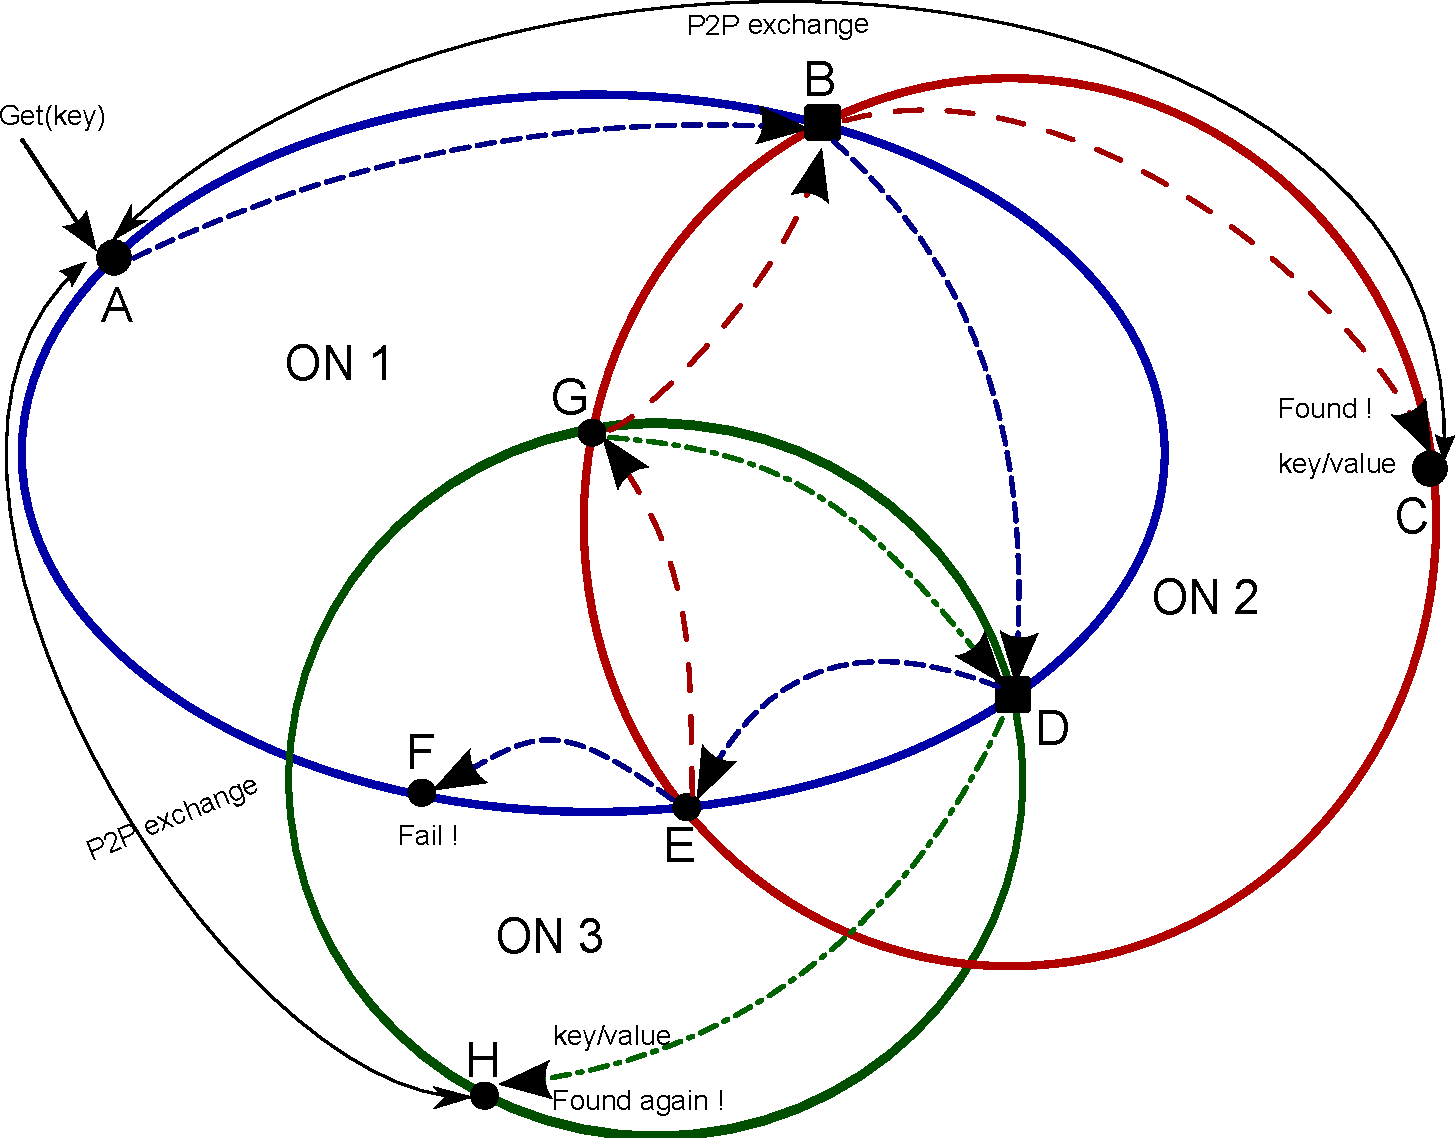
\includegraphics[width=\columnwidth]{fig/GET_into_other_ON.pdf}
  \caption{Routing across differents overlays\label{fig:example}}
  \end{figure}



  \begin{figure}
    \centering
    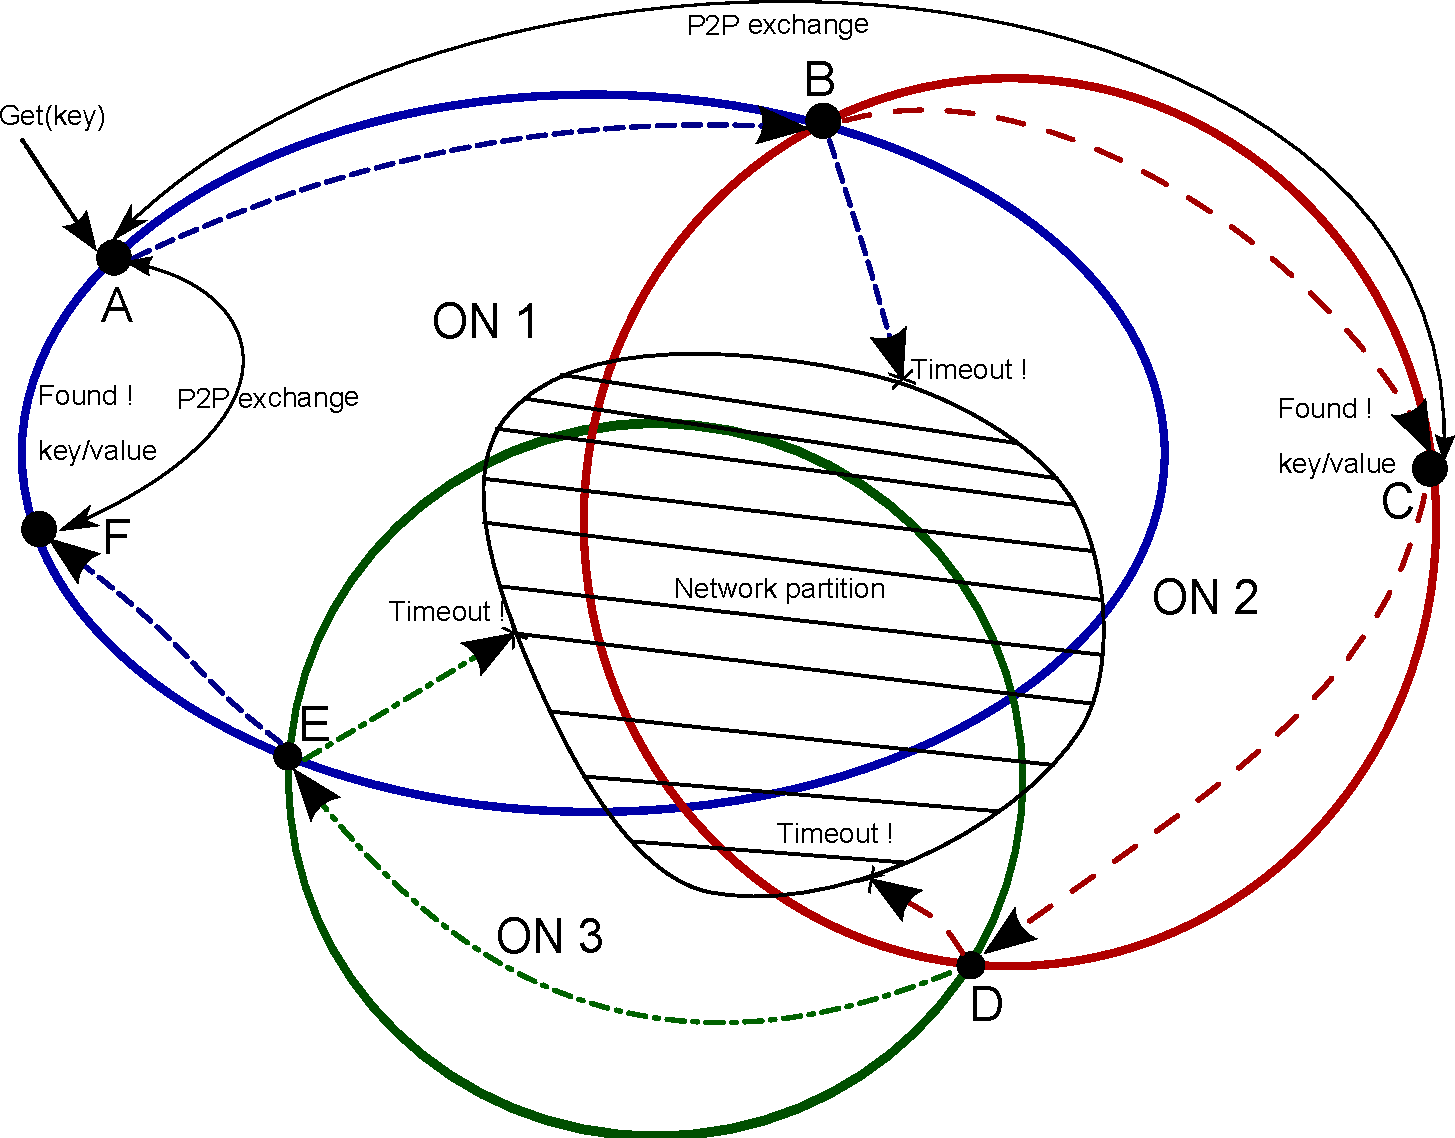
\includegraphics[width=\columnwidth]{fig/ON_with_network_partition.pdf}
    \caption{Dealing with a network partition \label{fig:example2}}
  \end{figure}


%% heart of the description
\subsection{Algorithms}
%
Figure~\ref{fig:lookup} presents the pseudo-code of the protocol using
message passing paradigm.

\subsubsection{The \texttt{GET} operation}
%
The {\tt GET} operation consists in finding the value of an object we
are seeking, provided its key. A node seeking an object sends an
\texttt{OPE(GET,key,\_)} message to an arbitrary node it knows. On
receipt (see lines~\ref{alg:ope}-\ref{alg:ope_end}), the node
generates a new tag {\tt tag} for this request that will be associated
with the query all along its path. The routing is then initiated with
a given TTL by sending an auxiliary {\tt FIND} message for this
request to the node itself; this message seeks the node(s) responsible
for the key sought in order to read the value (if it exists).

On receipt of a {\tt FIND} message (see
lines~\ref{alg:find}-\ref{alg:find_end}), the node checks the TTL and
the tag of the request before starting processing the request, and,
first, recording it as \emph{already processed} (``game over''
stategy). The retrieval process starts then locally, in two steps for
each intra-overlay the node belongs to: $(i)$ it checks if, according
to the particular retrieval algorithm of the intra-overlay, it is
itself assigned a range of keys containing {\tt key} (line
\ref{alg:test}), if this is the case, for this overlay, the retrieval
process ends and a {\tt FOUND} message is sent back to the initiator
of the request informing it that the potential value sought is stored
on this node (line~\ref{alg:send_found})). $(ii)$ if the node was not
responsible for the key in this particular overlay, it forwards the
request to the \emph{next hop} inside this intra-overlay, according to
the particular overlay's policy (line \ref{alg:find_end}).

% \Fr{}\Ce{ Parler de {\tt distrib\_mrr} as the function calculating the
% associative list ({\tt net-mrr}), ligne 2.04 (see web page for
% examples of how the function work)}

On receipt of such a {\tt FOUND} message --- recall that several
responses can be obtained for a request --- the initiator of the {\tt
  GET} request sends a {\tt READ\_TABLE} message to the responsible of
the key, basically to get the value of the key sought (see
lines~\ref{alg:get_code}-\ref{alg:get_code_end}).

\subsubsection{The \texttt{PUT} operation}
%
The {\tt PUT} operation is a declaration of a resource. Depending on
the purpose of the resource aggregation, the {\tt PUT} policy may
change:

\begin{itemize}
 \item If the purpose of the aggregation is to let each overlay keep
   the control on their information (with exclusive rights for
   writing and updating the information) while letting nodes from
   other overlay read this information, the {\tt PUT} operation will
   be performed independently within each overlay, each node
   declaring their resources to their intra-overlays. In this first
   case, the {\tt PUT} operation will not be different as in a set of
   intra-overlays without inter-connection, and corresponds to set
   the Maximum-Replication-Rate (MRR) to 0.

 \item If the purpose of the aggregation is to build a globally
   distributed information system, each node may declare its resources
   to a set of intra-overlays it may not belong to. In this last case,
   the {\tt PUT} operation involves mechanisms very similar to the
   {\tt GET} operation and the Maximum-Replication-Rate (MRR)
   different than zero tells how many copies we want to distribute in
   the inter-overlay. Line $2.04$ computes via the function {\tt
     distrib\_mrr}\footnote{Please refer to the Synapse web page for
     more information} the required values of MRR for a {\tt PUT}
   request, starting from both its current value and the number of
   intra-overlays the request will be forwarded to. Recall that MRR is
   ignored when the message is not a {\tt PUT} operation. In fact, a
   node declaring a resource will also seek nodes in the Synapses
   responsible for their resources. Once such location is found
   (similarly than for the {\tt GET} operation), the initiator of the
   request has just to send the value to be stored by the responsible
   nodes found. This is achieved by
   lines~\ref{alg:put_code}-\ref{alg:put_code_end}.

\end{itemize}

\subsubsection{The \texttt{JOIN} and \texttt{INVITE} operations}
%
The {\tt JOIN} message is sent by a node entering the network, upon a
reception of an {\tt INVITE} message. Please refer to
lines~\ref{alg:join_req}-\ref{alg:join_req_end} for invitation, and to
lines~\ref{alg:join_req_ok}-\ref{alg:join_req_ok_end} for join. The
intra-overlays in which a joining node will act can be chosen in
different ways. A peer receiving an invitation to join a network
through the {\tt INVITE} message sent by another node can evaluate,
via the {\tt good\_deal?}  social-based primitive, the relevance of
this invitation. If the invitation was positively evaluated, it can
send a {\tt JOIN} message to the peer that launched the
invitation. Upon receipt of a {\tt JOIN} message, a peer can decide,
again via the {\tt good\_deal?}  primitive, whether or not this join
is interesting for it.


% \paragraph{The \texttt{leave} operation.}

% The {\tt leave} operation differs from the others in the sense that no
% additional code is required, each leaving operation being normally
% handled by each overlay a node belongs to.


